% --- RSSM / PlaNet ---
% % --- Part C: RSSM (thread from Bierling 2025 Medium; figures from PlaNet PDF) ---
\begin{frame}[t]{RSSM: Motivation}
  \begin{itemize}\itemsep0.38em
    \item Purely deterministic RNNs (e.g., GRUs, LSTMs) struggle to represent multiple plausible futures in complex, stochastic environments.
    \item \textbf{Recurrent State Space Models (RSSM)} address this by combining:
      \begin{itemize}
        \item \textbf{Deterministic hidden state} $h_t$ (e.g., GRU): maintains long-term memory and context.
        \item \textbf{Stochastic state} $z_t$ (e.g., Gaussian): captures uncertainty and enables diverse possible futures.
      \end{itemize}
    \item This split allows RSSM to unify stable memory (for causality) and flexible modeling (for multi-modal, uncertain environments).
    \item Without the stochastic component, agents often \textbf{fail to learn} in partially observable or noisy tasks.
    \item Result: a flexible temporal representation for RL agents capable of handling uncertainty and representing many possible outcomes.
  \end{itemize}
\end{frame}

\begin{frame}[t]{RSSM: Architecture}
  \centering
  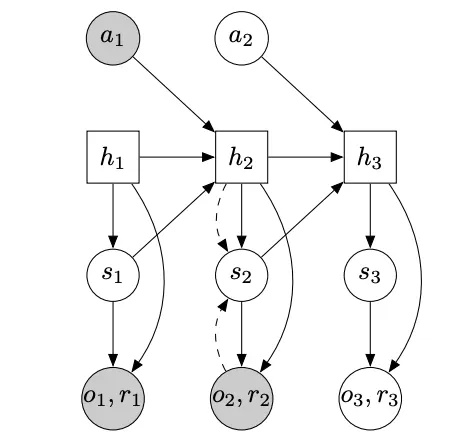
\includegraphics[width=0.65\linewidth,height=0.65\textheight,keepaspectratio]{images/world-models/rssm_architecture_diagram.png}\\[0.2em]
  {\scriptsize Recurrent State Space Model (RSSM). Circles are stochastic variables (filled when observed) and squares are deterministic variables; solid lines denote the generative process, dashed lines the inference model. A mixed deterministic--stochastic model. Source: \href{https://arxiv.org/pdf/1811.04551}{PlaNet, arXiv:1811.04551}.}
\end{frame}

\begin{frame}[t]{RSSM: Dynamics}
  \begin{itemize}
    \item \textbf{Posterior transition (training):} Updates stochastic state using real observation
    \[ z_t \sim q_\phi(z_t \mid h_t, x_t) \]
    \item \textbf{Prior transition (imagination):} Predicts next latent state without observation,
    \[ z_t \sim p_\theta(z_t \mid h_t) \]
    \item \textbf{Training objective:} the model learns by reconstructing images, predicting rewards, and keeping its imagined predictions close to what really happened, using an ELBO-style loss (next slide).
    \item This ensures that planning in latent space is meaningful: predictions made during ``imagination'' are grounded in real transitions.
  \end{itemize}
\end{frame}

\begin{frame}[t]{RSSM: Training Objective}
  The same ELBO as the VAE, unrolled through time, with a reward head added:
  \begin{equation*}
    \max \;\; \mathbb{E}_{q}\!\left[\sum_t \Big(
      \underbrace{\ln p(x_t \mid h_t, z_t)}_{\text{reconstruction}}
      + \underbrace{\ln p(r_t \mid h_t, z_t)}_{\text{reward prediction}}
      - \beta\, \underbrace{\mathrm{KL}\!\big(q(z_t \mid h_t, x_t)\,\|\,p(z_t \mid h_t)\big)}_{\text{imagination matches reality}}
    \Big)\right]
  \end{equation*}
  \begin{itemize}\itemsep0.25em
    \item \textbf{Reconstruction} grounds the latent state in observations.
    \item The \textbf{reward head} makes latent rollouts useful for planning and RL.
    \item The \textbf{KL term} pulls the prior (used during imagination) toward the posterior (informed by real observations), so imagined futures stay realistic.
  \end{itemize}
\end{frame}

% --- PlaNet: planning with the learned model ---
\begin{frame}[t]{PlaNet: Planning in Latent Space}
  \begin{itemize}\itemsep0.28em
    \item \textbf{PlaNet} (Hafner et al., 2019) pairs the RSSM with \textbf{online planning}; there is no policy network at all.
    \item At each step: sample candidate action sequences, roll them out in \textbf{latent space}, score them with the predicted rewards, and refine with the \textbf{cross-entropy method (CEM)}; execute the first action and replan.
    \item This is the same CEM / model-predictive-control loop V-JEPA 2-AC used in the JEPA lecture; PlaNet did it with an ELBO-trained generative model and a reward head instead of goal images.
    \item Learns image-based control tasks with far fewer environment interactions than model-free baselines.
    \item Two costs: planning at every step is expensive, and CEM has no value estimate beyond its horizon. \textbf{Dreamer} fixes both.
  \end{itemize}
\end{frame}
